\documentclass[acmlarge]{acmart}

\setcopyright{acmcopyright}
\copyrightyear{2020}
\acmNumber{4}
\acmMonth{8}

\usepackage{listings}
\usepackage[section]{placeins}
\usepackage{multirow}
\usepackage{pgfplots}
\usepackage{yfonts}
\usepackage{subcaption}

\pgfplotsset{width=7cm,compat=1.8}

\lstdefinelanguage{ocanren}{
keywords={run, conde, fresh, let, in, match, with, when, class, type,
object, method, of, rec, until, while, not, do, done, as, val, inherit,
new, module, sig, deriving, datatype, struct, if, then, else, open, private, virtual, include, success, failure,
true, false},
sensitive=true,
commentstyle=\small\itshape\ttfamily,
keywordstyle=\textbf,%\ttfamily\underline,
identifierstyle=\ttfamily,
basewidth={0.5em,0.5em},
columns=fixed,
mathescape=true,
fontadjust=true,
literate={fun}{{$\lambda$}}1 {->}{{$\to$}}3 {===}{{$\equiv$}}1 {=/=}{{$\not\equiv$}}1 {|>}{{$\triangleright$}}3 {\\/}{{$\vee$}}2 {/\\}{{$\wedge$}}2 {^}{{$\uparrow$}}1,
morecomment=[s]{(*}{*)}
}

\lstset{
language=ocanren
}

\newcommand{\ruleno}[1]{\mbox{[\textsc{#1}]}}
\newcommand{\rulen}[1]{[\textsc{#1}]}
\newcommand{\mk}[0]{\textsc{miniKanren}}
\newcommand{\inbr}[1]{\langle #1 \rangle}

\begin{document}

\title{Fair relational conjunction}

\author{Petr Lozov}
\email{lozov.peter@gmail.com}        

\author{Dmitry Boulytchev}
\email{dboulytchev@math.spbu.ru}    

\affiliation{
  \institution{Saint Petersburg State University}
  \country{Russia}                   
}

\affiliation{
  \institution{JetBrains Research}   
  \country{Russia}                   
}

\begin{abstract}
  Abstract will be here.
\end{abstract}

\begin{CCSXML}
<ccs2012>
<concept>
<concept_id>10011007.10011006.10011008.10011009.10011015</concept_id>
<concept_desc>Software and its engineering~Constraint and logic languages</concept_desc>
<concept_significance>500</concept_significance>
</concept>
</ccs2012>
\end{CCSXML}

\ccsdesc[500]{Software and its engineering~Constraint and logic languages}

\keywords{relational programming, evaluation strategies}

\maketitle

\section{Introduction}

Relational programming is an approach, based on the idea of describing programs not as functions, but 
as relations, without distinguishing between the arguments and the result value. This technique makes it 
possible to ``query'' programs in various ways, for example, to execute them ``backwards'', finding
all sets of arguments for a given result. Relational behavior can be reproduced using a number of
logic programming languages, such as Prolog, Mercury~\cite{Mercury}, 
or Curry~\cite{Curry}. 
There is also a family of embedded DSLs, specifically designed for writing declarative relational
programs that originates from \miniKanren~\cite{TRS}. \miniKanren is a minimalistic 
declarative language, initially developed for Scheme/Racket. The smallest implementation of \miniKanren 
is reported to comprise of only 40 LOC~\cite{MicroKanren,2016}; there are also more elaborate versions, including
\miniKanren with constraints~\cite{CKanren,CKanren1}, user-assisted search~\cite{Guided}, nominal unification~\cite{AlphaKanren},
etc. Due to its simplicity, \miniKanren was implemented for more than 50 other languages, such as
Haskell, Go, Smalltalk, and OCaml. In a nutshell, miniKanren introduces a minimalistic set of constructs to describe
relations over a set of syntactic terms, thus providing the same expressivity as a pure core of conventional
logic programming\footnote{A detailed miniKanren to Prolog comparison can be found at \url{http://minikanren.org/minikanren-and-prolog.html}}. 

\miniKanren has proven to be a useful tool to provide elegant solutions for various problems, otherwise considered as
non-trivial~\cite{WillThesis}. One of the most promising areas of application for \miniKanren is the implementation of
\emph{relational interpreters}. Such interpreters are capable not only to interpret programs in various directions, but also
to infer programs on the basis of expected input-output specification~\cite{Untagged}.

Being quite simple and easy to use by design, in implementation \miniKanren introduces some subtleties. Under the hood, \miniKanren 
uses a complete interleaving search~\cite{Search}. This search is guaranteed to find all existing solutions; however, it can diverge, when no 
solution exists. In reality, this amounts to divergence in a number of important cases~--- for example, when a program is asked to 
return \emph{all} existing solutions, or when the number of requested solutions exceeds the number of existing ones.
It is often possible to refactor the specification of a concrete query to avoid the divergence, but this has to be done for every execution
``direction'' of interest that compromises the idea of fully declarative relational programming.

The specifications that do not diverge even when no solutions exist, are called \emph{refutationally complete}~\cite{WillThesis}. Writing 
refutationally complete relational specifications nowadays requires knowledge of \miniKanren implementation intrinsics, and is not always
possible due to the undecidability of the fundamental computability problems. However, by developing a more advanced search it is possible
to make more specifications refutationally complete.

In this work we address one particular problem that often leads to refutational incompleteness~--- the non-commutativity of
conjunction. We present an optimization technique that is based on a certain non-termination test. Our optimization
is \emph{online} (performed during the search), \emph{non-intrusive} (does not introduce new constructs and does not require
any changes to be made to the existing specifications), and \emph{conservative} (applied only when the divergence
is detected). We prove that for the queries that return a finite number of answers, our optimization preserves convergence. 
We also demonstrate the application of the optimization for a number of interesting and important problems.

We express our gratitude to William Byrd and the reviwers of this paper for their constructive remarks and suggestions.


\section{Directed Conjunction}
\label{sec:directed}

% В этом разделе мы рассмотрим реляционный язык miniKanren с классической направленной конъюнкцией, изучим достоинства и недостатки направленной конъюнкции на примерах.
In this section we consider the classic directed conjunction in the original \mk and demonstrate its advantages and drawbacks on examples. 

% В языке miniKanren между операциями дизъюнкции и конъюнкции есть существенная разница. Дизъюнкция вычисляет свои аргументы попеременно, что приводит к равномерному вычислению двух дизъюнктов. Такого поведения дизъюнкции достаточно для полного поиска ответов. Конъюнкция же извлекает ответы из первого конъюнкта, на которых вычисляет второй конъюнкт. С одной стороны, такая конъюнкция проста в реализации и позволяет явно задать порядок исполнения конъюнктов. С другой стороны, эта конъюнкция ассиметрична. Более того, она может сходиться при одном порядке конъюнктов, но расходиться при другом. Например, отнонение freeze в зависимости от аргумента либо сходится за один шаг рекурсии, либо расходится. Тогда конъюнкция вида (=== /\ freeze) сходится, но при перестановке конъюнктов мы получаем расхождение. Действительно, в первом случае первый конъюнкт производит ровно один ответ, который противоречит унификации в теле отношения freeze. Во втором случае отношение freeze разойдется и не произведет ни одного ответа и второй конъюнкт вычислен не будет. 

In \mk there is a significant difference between disjunction and conjunction evaluation strategy. The arguments of disjunction are evaluated
in an \emph{interleaving} manner, switching elementary evaluation steps between disjuncts, which provides the completeness of the search.
Conjunction, on the other hand, waits for the answers from the first conjunct and then calculates the second conjunct in the context of each answer.

On the one hand, this strategy is easy to implement and allows one to explicitly specify the order of evaluation when this order is essential.
On the other hand, the strategy amounts to non-commutativity: the convergence of a conjunction can depend on the order of its arguments.
For example, the relation

\begin{lstlisting}
   let rec freeze$^o$ x = x ===  true /\ freeze$^o$ x
\end{lstlisting}

\noindent either converges in one recursion step or diverges. The conjunction \lstinline{(x === false/\ freeze$^o$ x)} converges, but the same conjunction with the reverse order of conjuncts
\lstinline{(freeze$^o$ x /\ x === false)} diverges. Indeed, in the first case the first conjunct produces exactly one answer which contradicts the unification in the body
of \lstinline{freeze$^o$}. In the second case the relation \lstinline{freeze$^o$} diverges and does not produce any answer. As a result we will never begin to evaluate the second conjunct.

\begin{figure}[h!]
\centering
\begin{tabular}{cp{3cm}c}
\begin{lstlisting}%[numbers=left,numberstyle=\small]
let rec append$^o$ x y xy =
  (x === [] /\ y === xy) \/
  fresh (e xs xys) (
    x === e : xs /\ 
    xs === e : xys /\ 
    append$^o$ xs y xys)
\end{lstlisting}
& &
\begin{lstlisting}%[firstnumber=7,numbers=left,numberstyle=\small,escapeinside={@}{@}]
let rec revers$^o$ x y =
  (x === [] /\ y === []) \/
  fresh (e xs ys) (
    x === e : xs /\ 
@\label{fair:reverso-call}@    revers$^o$ xs ys /\
@\label{fair:appendo-call}@    append$^o$ ys [e] y)
\end{lstlisting}
\end{tabular}

\caption{Relational list reversing}
\label{fair:lst-reverso}
\end{figure}

% Конечно, данная проблема решается правилом, которому нужно следовать при работе с miniKanren: унификацию нужно ставить самым левым конъюнктом. Но иногда оба конъюнктв являются вызовами отношений. В частности отношение обращения списка revers, которое связывает произвольный список со списком, содержащим элементы в обратном порядке. В этом отношении есть пара конъюнктов append и revers. При таком порядке вызов revers сходится, но при обратном порядке он расходится. Более того при обратном порядке снижается скорость вычисления ответа. 
The problem in this particular example can be alleviated by using a conventional rule for \mk, which says that unifications must be moved first in a cluster of conjunctions.
But the rule does not work for clusters with more than one relational call. Consider, for instance, the relation \lstinline{revers$^o$} (Fig.~\ref{fair:lst-reverso}), which associates
an arbitrary list with the list containing the same elements in reverse order. In this relation we can see a couple of conjuncts: \lstinline{revers$^o$} on line~\ref{fair:reverso-call} and
\lstinline{append$^o$} on line~\ref{fair:appendo-call}. With this particular order, the call \lstinline{(revers$^o$ [1, 2, 3] q)} converges, but in reverse order it diverges after an answer
is found. Moreover, the reverse order negatively affects the performance of the answer evaluation.

% В то же время, вызов revers при заданном порядке конъюнктов расходится, а при обратном сходится. В результате мы бы хотели разный порядок конъюнктов в зависимости от конкретных аргументов.

At the same time the call \lstinline{(revers$^o$ q [1, 2, 3])} for a given order of conjuncts diverges, and for the reverse order it converges. As a result a
different order of conjuncts is desirable depending on their runtime values.

% В следующих разделах мы предлжожим подход, который будет определять оптимальный порядок автоматически во время исполнения программы.
In the following sections we describe an approach for automatically determining a ``good'' order during program evaluation.

\section{Semantics of directed conjunction}
% В этом разделе мы введем операционную семантику малого шага для определения поведения оригинального miniKanren с направленной конъюнкцией.
In this section we introduce the small step operational semantics to define the behavior of the original \mk~ with directional conjunction. 

% Отметим, что на данный момент существует сертифицированная семантика языка miniKanren, однако она делает большие различия между первым и вторым конъюнктом, что сильно усложняет задачу перестановки конъюнктов в процессе исполнения программы. Поэтому для данной работы мы разработали новую семантику, которая изначально не делает различий между конъюнктами.

Note, at the moment there is certified semantics~\cite{fair:semantics} of the \mk, however, it makes great differences between the first and second conjuncts, which greatly complicates the task of rearranging the conjuncts in the process of program evaluation. 
Therefore, for this research, we have developed a new semantics that initially does not distinguish between conjuncts.

% Семантика, которую мы предлагаем, основана на развертке вызовов отношений. На каждом шаге в текущем состоянии программы выбирается некоторый вызов, который разворачивается. Этот процесс продолжается, пока в текущем представлении остаются вызовы. Ниже мы опишим эту семантику более формально.

The semantics that we offer are based on unfolding of the relation calls.
At each step, we select a call from the current state of the program. 
We are unfolding this call.
This process continues while calls remain in the state of program. 
Below we define this semantics more formally.

% Прежде всего мы определим синтаксис языка \mk на изображении 2. Конструкторы с арностью являются стандартным представлением данных. Синтаксические переменные необходимы для описания аргументов отношения и свежих переменных в операции fresh. Семантические переменные в исходной программе отсутствуют, однако они вводятся при исполнении операции fresh. Из конструкторов, синтаксический переменных и семантических переменных мы определили множество синтаксических термов и множество семантических переменных. Также мы определили множество имен отношений с арностью. Далее, мы определили цели. Цели являются унификацией термов, дизъюнкцией, конъюнкцией введением свежей переменной или вызовом отношения. Наконец мы определяем множество отношений. Каждое отношение состоит из имени с арностью, списка имен переменных и тела отношения.

First of all, we define the syntax of the language \mk~ in figure~\ref{fair:syntax}.
Constructors with arity $\mathcal{C}$ are a standard representation of data.
Syntax variables $\mathcal{X}$ are needed to describe the relation arguments and the fresh variables in the \lstinline{fresh} operation.
There are no semantic variables $\mathcal{A}$ in the source program, but they are introduced during the evaluation of the \lstinline{fresh} operation. 
We define set of syntax terms $\mathcal{T}_\mathcal{X}$ and set of semantic terms $\mathcal{T}_\mathcal{A}$ using the constructors, syntax variables and semantic variables. 
Also we define set of relation names with arity $\mathcal{F}$.
Next, we describe goals $\mathcal{G}$. Goals are the unification of terms, disjunction, conjunction, the introduction of a fresh variable, or the call of a relation. 
Finally, we define the set of relations $\mathcal{S}$. Each relation consists of the name with arity, the list of variable names, and the body of the relation.

\begin{figure}[h]
\[
  \begin{array}{rcll}
     \mathcal{C} & = & \{ C_1^{k_1}, C_2^{k_2}, \ldots \} 
     & \mbox{constructors with arities} 
     \\
     \mathcal{X} & = & \{x_1, x_2, \ldots \} 
     & \mbox{syntax variables} 
     \\
     \mathcal{A} & = & \{\alpha_1, \alpha_2, \ldots \} 
     & \mbox{semantic variables} 
     \\
     \mathcal{T}_\mathcal{X} & = & \mathcal{X} \mid C_i^{k_i}(\mathcal{T}_\mathcal{X}^1, \ldots, \mathcal{T}_\mathcal{X}^{k_i})
     & \mbox{syntax terms} 
     \\
     \mathcal{T}_\mathcal{A} & = & \mathcal{A} \mid C_i^{k_i}(\mathcal{T}_\mathcal{A}^1, \ldots, \mathcal{T}_\mathcal{A}^{k_i})
     & \mbox{semantic terms} 
     \\
     \mathcal{F} & = & \{F_1^{k_1}, F_2^{k_2}, \ldots \} 
     & \mbox{names of relations with arities} 
     \\
     \mathcal{G} & =    & \mathcal{T}_\mathcal{X} \equiv \mathcal{T}_\mathcal{X} & \mbox{unification} \\
                 & \mid & \mathcal{G} \lor \mathcal{G} & \mbox{disjunction} \\
                 & \mid & \mathcal{G} \land \mathcal{G} & \mbox{conjunction} \\
                 & \mid & \mbox{\lstinline|fresh|} \; (\mathcal{X}) \; \mathcal{G} & \mbox{fresh variable introduction} \\
                 & \mid &  F_i^{k_i}(\mathcal{T}_\mathcal{X}^1, \ldots, \mathcal{T}_\mathcal{X}^{k_i}) & \mbox{relation call} \\
    \mathcal{S} & = &F_i^{k_i} = \lambda \mathcal{X}_1 \ldots \mathcal{X}_n. \; \mathcal{G} & \mbox{relations}
  \end{array}
\]
    \caption{The syntax of the relational language}
    \label{fair:syntax}
\end{figure}

% Помимо синтаксиса нам понадбится промежуточное состояние реляционной программы. Это состояние является деревом дизъюнкций. Внутренние узел \circ соотвествует дизъюнкции двух состояний-потомков. Его листья содержат промежуточные подстановки, индекс семантических переменных i, и список вызовов. Подстановка --- это отображение из семантических переменных в семантические термы. Оно содержит информацию о текущих переменных и обновляется при исполнении унификаций. Индекс семантических переменных необходим для исполнения операции fresh, которая вводит семантическую переменную с новым индексом. Список вызовов содержит вызовы отношений c_i, которые необходимо довычислить в этой ветке. Список \epsilon соответствует пустому списку, а оператор (:) определяет добавление вызова в список.

In addition to the syntax, we need an intermediate state of the relational program
\[
\textgoth{T} = \inbr{\sigma, i, c_1 : \ldots : c_n : \epsilon} \mid \textgoth{T} \circ \textgoth{T} \mbox{, where } c_i = F_i^{k_i}(t_\mathcal{A}^1, \ldots, t_\mathcal{A}^{k_i}).
\]
This state is a disjunction tree. The internal node $(\circ)$ corresponds to the disjunction of two descendant states.
Its leaves contain intermediate substitutions $\sigma$, counter of semantic variables $i$ and list of calls. 
Substitution $\sigma$ is mapping from semantic variables to semantic terms. 
It contains information about the current variables and is updated during the evaluation of unifications. 
The counter of semantic variables is necessary to evaluate the \lstinline{fresh} operation, which introduces a semantic variable with a new counter.
List of calls contains calls $c_i$ that must be evaluated in this branch.
The list $\epsilon$ corresponds to an empty list, and the operator $(:)$ determines the addition of a call to the list.

% Мы расширим множество состояний пустым состоянием, которое соотвествует завершению вычисления. 

We expand the set of states with an empty state
\[
\bar{\textgoth{T}} = \emptyset \mid \textgoth{T},
\]
which corresponds to the completion of the evaluation.

% Также мы введем две вспомогательных функции для работы с состоянием программы. Первая функция union (изображение 3) производит объединение двух состояний.
Also we introduce two auxiliary functions for working with the program state. The first function $union$ (fig.~\ref{fair:union-semantics}) combines two extended states.

\begin{figure}[h!]
\[
union(T_1, T_2) =
\left\{
\begin{array}{rl}
T_2, & \mbox{if } T_1 = \emptyset \\
T_1, & \mbox{if } T_1 \not= \emptyset \mbox{ and } T_2 = \emptyset \\
(T_1 \circ T_2), & \mbox{otherwise}
\end{array}
\right.
\]
\caption{Auxiliary function $union$}
\label{fair:union-semantics}
\end{figure}

% Если одно из состояний пустое, функция union вернёт второе. Если оба состояния не пусты, то функция вернёт объединенное состояние.

If one of the states is empty, the function $union$ returns the second state. If both states are not empty, then the function returns the combined state.

\begin{figure}[h!]
\[
push(C, T) =
\left\{
\begin{array}{rl}
\inbr{\sigma, i, c_1 : \ldots : c_i : \bar{c_1} : \ldots : \bar{c_k} : cs}, & \mbox{if } T = \inbr{\sigma, i, \bar{c_1} : \ldots : \bar{c_k} : \epsilon} \mbox{ and } C = c_1 : \ldots : c_i : \Box : cs \\
(push(C, T_1) \circ push(C, T_2)), & \mbox{if } T = (T_1 \circ T_2)
\end{array}
\right.
\]
\caption{Auxiliary function $push$}
\label{fair:push-semantics}
\end{figure}

% Следующая вспомогательная функция push (изображение 4) необходима для конструирования состояние после развертки. Первый аргумент --- это список вызовов, который содержит дырку. На этом месте стоял вызов, который мы развернули. Второй аргумент --- состояние, которое является результатом развертки. Данная функция рекурсивно проходит по состоянию, а в каждом листе объединяет вызовы с дыкой и вызовы из листа. 

The following auxiliary push function (fig.~\ref{fair:push-semantics}) is needed to construct the state after the unfolding. 
The first argument of this function is a call list that contains a hole. 
The hole corresponds to the position of the call that we unfold. 
The second argument is the state that results from the unfolding. 
This function recursively traverse by state, and for any leafs it combines calls with hole and leaf calls.

% Теперь мы определим семантику для операции развертки. Эта семантика приобразовывает вызов отношения и подстановку в состояние, которое соответствует телу этого отношения. Так как развертка вызова --- конечный процесс, мы можем описать развертку как семантику большого шага.
Now we define the semantics for the unfolding operation. This semantics (fig.~\ref{fair:unfolding-semantics}) evaluates a call of a relation and a substitution into a state that corresponds to the body of this relation. Since the call unfolding is the finite process, we can describe the unfolding as the big step semantics.

\begin{figure}[h!]
\[\begin{array}{cr}

\dfrac{ F = \lambda \bar{x}. b \qquad \inbr{\sigma, i, \epsilon} \vdash b[\bar{x} \leftarrow \bar{t}] \leadsto T}
      {(\sigma, i) \vdash F(\bar{t}) \Rightarrow T}
&     \ruleno{Unfold} \\[3mm]
\dfrac{\not\exists \, mgu(t_1, t_2, \sigma)}
      {\inbr{\sigma, i, cs} \vdash (t_1 \equiv t_2) \leadsto \emptyset}
&     \ruleno{UnifyFail}  \\[3mm]
\dfrac{\bar\sigma = mgu(t_1, t_2, \sigma)}
      {\inbr{\sigma, i, cs} \vdash (t_1 \equiv t_2) \leadsto \inbr{\bar\sigma, i, cs}}
&     \ruleno{UnifySuccess}  \\[3mm]
      {\inbr{\sigma, i, cs} \vdash F(\bar{t}) \leadsto \inbr{ \sigma, i, F(\bar{t}) : cs}}
&     \ruleno{Call} \\[2mm]
\dfrac{\inbr{\sigma, i+1, cs} \vdash g[x \leftarrow \alpha_i] \leadsto T}
      {\inbr{\sigma, i, cs} \vdash (\mbox{\lstinline|fresh|} \, x. \, g) \leadsto T}
&     \ruleno{Fresh}  \\[3mm]
\dfrac{\inbr{\sigma, i, cs} \vdash g_1 \leadsto T_1 \qquad \inbr{\sigma, i, cs} \vdash g_2 \leadsto T_1}
      {\inbr{\sigma, i, cs} \vdash (g_1 \lor g_2) \leadsto union(T_1, T_2)}
&     \ruleno{DisjGoal}  \\[3mm]
\dfrac{g \not= g_1 \lor g_2 \qquad T_1 \vdash g \leadsto T_3 \qquad T_2 \vdash g \leadsto T_4}
      {(T_1 \circ T_2) \vdash g \leadsto union(T_3, T_4)}
&     \ruleno{DisjState}  \\[3mm]
\dfrac{\inbr{\sigma, i, cs} \vdash g_1 \leadsto \emptyset}
      {\inbr{\sigma, i, cs} \vdash (g_1 \land g_2) \leadsto \emptyset}
&     \ruleno{ConjFail}  \\[3mm]
\dfrac{\inbr{\sigma, i, cs} \vdash g_1 \leadsto T \qquad T \vdash g_2 \leadsto \bar{T}}
      {\inbr{\sigma, i, cs} \vdash (g_1 \land g_2) \leadsto \bar{T}}
&     \ruleno{ConjSuccess}  \\[3mm]
\end{array}\]

\caption{Big step semantics of Unfolding}
\label{fair:unfolding-semantics}
\end{figure}

% Правило [Unfold] является внешним. Поэтому оно единственное содержит символ =>. Оно запускает процесс развертки вызова F(t) в контексте подстановки и счетчика семантических переменных. Прежде всего, вызов заменяется на тело отношения. Производится подстановка аргументов, инициализируется состояние. Далее запускается преобразование тела отношения в соответствующее состояние.
The \rulen{Unfold} rule is external. 
Therefore, it only contains the symbol ($\Rightarrow$). 
It starts the unfolding process of call $F$ with list of arguments $\bar{t}$ in the context of substitution $\sigma$ and the counter of semantic variables $i$.
First of all, the call $F$ is replaced by the body $b$ of the relation. Also the arguments $\bar{x}$ are substituted by terms $\bar{t}$, the state $\inbr{\sigma, i, \epsilon}$ is initialized. Next, we evaluate the relation body into the correspond state using the rest of rules.

% Правила [UnifyFail] и [UnifySuccess] исполняют унификацию. Если существует ноиболее общий унификатор (MGU), то мы применяем правило [UnifySuccess], которое обновляет подстановку. Если MGU не существует, то мы применияем правило [UnifyFail], что приводи к пустому состоянию.
The rules \rulen{UnifyFail} and \rulen{UnifySuccess} perform unification. If the most common unifier (MGU) exists, then we apply the \rulen{UnifySuccess} rule, which updates the substitution $\sigma$. If the MGU does not exist, then we apply the \rulen{UnifyFail} rule, which leads to an empty state.

% Так как развертка должна развернуть вызов ровно один раз, все вложенные вызовы мы оставляем без изменений. Данное поведение описано в правиле [Call]. Вложенный вызов не вычисляется, а помещаяется в список вызовов состояния.
Since this semantics should unfold the call exactly once, we leave all the nested calls unchanged. This behavior is described in the \rulen{Call} rule. The nested call is not evaluated, but placed on the call list, which is contained into the state.

% Правило [Fresh] соответствует введению свежей переменной. В данном правиле мы заменяем синтаксическую переменную на семантическую переменную. Также мы увеличиваем счетчик семантических переменных. 
The \rulen{Fresh} rule corresponds to the introduction of a fresh variable. In this rule, we replace a syntax variable $x$ with a semantic variable $\alpha_i$. We also increment the counter of semantic variables.

% Правила [DisjGoal] и [DisjState] необходимы для исполнения дизъюнкции. Первое правило вычисляет оба дизъюнкта и объединяет их в новое состояние с помощью вспомогательной функции union. Второе правило обрабатывает дизъюнкцию, содержащуюся в состоянии. Как и в первом правиле мы производим два независимых вычисления, а затем объединяем результаты в новое состоения.
The rules \rulen{DisjGoal} and \rulen{DisjState} are required to evaluate a disjunction. The first rule evaluates both disjuncts and combines them into a new state using the auxiliary function $union$. The second rule handles a disjunction which is contain in the state. As in the previous rule, we perform two independent evaluations, and then combine the results in a new state.

% Оставшиеся два правила описывают вычисление конъюнкции. Если первый конъюнкт вычислился в пустое состояние, то мы применяем правило [ConjFail], которое возвращает пустое состояние как результат вычисления всей конъюнкции. В противном случае вычисляем первый конъюнкт в состояние T, а затем вычисляем второй конъюнкт в контесте состояния T. Таким образом, второй конъюнкт будет исполнен в контексте всех листьев состояния Т.
The last two rules \rulen{ConjFail} and \rulen{ConjSuccess} describe the evaluation of conjunction. If the first conjunct is calculated to an empty state, then we apply the \rulen{ConjFail} rule, which returns an empty state as a result of calculating the entire conjunction. Otherwise, we evaluate the first conjunct to state $T$, and then we evaluate the second conjunct in the context of state $T$. Thus, the second conjunct will be evaluated in the context of all leaves of the state $T$.

% Теперь у нас есть всё необходимое, чтобы определить семанику реляционного языка с направленной конъюнкцией. Данная семантика малого шага последовательно преобразовывает состояние и периодически производит ответы. Так как \mk недетеримированный язык, количество ответов, которое может получиться неограничено. Если в процессе исполнения программы будет обнаружен ответ, он будет помещён над символом перехода (->). В противном случае над символом перехода будет помещен \circ.

Now we have everything we need to define the semantics of a relational language with directed conjunction (fig.~\ref{fair:classic-semantics}). This small step semantics sequentially evaluates a state and periodically produces substitutions which are answers. Since \mk is a non-deterministic language, the number of answers that can be obtained is unlimited. If an answer is found during program evaluation, it will be placed above the transition symbol ($\xrightarrow{}$). Otherwise, ($\circ$) will be placed above the transition symbol.

\begin{figure}[h!]
\[\begin{array}{cr}

      {\inbr{\sigma, i, \epsilon} \xrightarrow{\sigma} \emptyset}  
&     \ruleno{Answer} \\[2mm]
\dfrac{(\sigma, i) \vdash c \Rightarrow T}
      {\inbr{\sigma, i, c : cs} \xrightarrow{\circ} push(\Box : cs, T)}
&     \ruleno{ConjUnfold} \\[2mm]
\dfrac{T_1 \xrightarrow{\alpha} \emptyset}
      {(T_1 \lor T_2) \xrightarrow{\alpha} T_2}
&     \ruleno{Disj} \\[4mm]
\dfrac{T_1 \xrightarrow{\alpha} \bar{T_1}}
      {(T_1 \lor T_2) \xrightarrow{\alpha} (T_2 \lor\bar{T_1})}
&     \ruleno{DisjStep} \\[4mm]
\end{array}\]
\caption{Semantics with directed conjunction}
\label{fair:classic-semantics}
\end{figure}

% Если текущее состояние является листом и не содержит вызовов, значит мы получили ответ. В этом случае мы применяем правило [Answer].
If the current state is a leaf and does not contain calls, then we got an answer. In this case, we apply the rule \rulen{Answer}.

% Если текущее состояние является листом, но содержит хотя бы один вызов, мы применяем правило [ConjUnfold]. Оно производит развертку самого левого вызова. Затем мы конструируем новое состояние из оставшищся вызовов и результата развертки с помощью функции push.
Also, if the current state is a leaf but contains at least one call, we apply the \rulen{ConjUnfold} rule. In this case we unfold the leftmost call $c$. Then we construct a new state from the remaining calls $cs$ and the unfolding result $T$ using the function $push$.

% Наконец, если текущее состояние является дизюнкцией, то мы производим вычисление в левом дизъюнкте T_1. В зависимости от результата мы приминяем или правило [Disj], или правило [DisjStep]. Первое правило соответствует пустому состоянию и возвращает второй дизъюнкт в качестве результата. Второе правило соответствует непустому состоянию и возвращает новое сотояние (T_2 \circ T_1). Перестановка дизъюнктов --- необходимое действие, которое называется интерливинг. Оно гарантирует полноту поиска.
Finally, if the current state is a disjunction, then we evaluate the left disjunct $T_1$. We apply either the \rulen{Disj} rule or the \rulen{DisjStep} rule depending on the result of evaluation the left disjunct. The first rule corresponds to an empty state and returns the second disjunct $T_2$ as a result. The second rule corresponds to a non-empty state and returns a new state ($T_2 \circ \bar{T_1}$). Rearrangement of disjuncts is a necessary action called interleaving~\cite{fair:interleaving}. It guarantees the completeness of the search.

% Для того чтобы сделать начальное состояние из вызова c, нам необходимо заменить в нем все синтаксические переменные на семантические. Тогда мы получим
In order to make the initial state from a call $c$, we need to replace all syntactic variables in it with semantic ones. Then we get
\[
\inbr{\{\}, n, c[x_0 \leftarrow \alpha_0, \ldots, x_{n-1} \leftarrow \alpha_{n-1}] : \epsilon}.
\]

% Данная семантика отличается от сертифицированной семантики и классических реализаций прежде всего размером шага. Операция развертки выполняет множество действий подряд, а в классическом случае после каждой элементарного действия выполняется интерливинг. Однако, общие черты данная семантика сохранила: дизъюнкты меняют порядок после каждого unfolding, а конъюнкты выполняются строго слева направо.
This semantics differs from certified semantics and classical implementations primarily in step size. The unfolding operation performs many actions in a row. But in the classic case, interleaving is performed after each elementary action. However, this semantics has retained common features: disjuncts change order after each step, and conjunctions are evaluated strictly from left to right. 


\begin{comment}
\[
\begin{array}{l}
\inbr{\{\}, 1, \mbox{\lstinline{revers}}^o \, [1] \; \alpha_0 : \epsilon} 
\xrightarrow{\circ} \\
\inbr{\{\alpha_1 = 1; \alpha_2 = []\}, 4, \mbox{\lstinline{revers}}^o \, \alpha_2 \; \alpha_3 : \mbox{\lstinline{append}}^o \, \alpha_3 \; [\alpha_1] \; \alpha_0 : \epsilon}
\xrightarrow{\circ} \\
\inbr{\{\alpha_1 = 1; \alpha_2 = []; \alpha_3 = []\}, 4, \mbox{\lstinline{append}}^o \, \alpha_3 \; [\alpha_1] \; \alpha_0 : \epsilon} 
\xrightarrow{\circ} \\
\inbr{\{\alpha_1 = 1; \alpha_2 = []; \alpha_3 = []\; \alpha_0 = [\alpha_1]\}, \epsilon}
\xrightarrow{\{\alpha_1 = 1; \alpha_2 = []; \alpha_3 = []\; \alpha_0 = [\alpha_1]\}} \emptyset
\end{array}
\]
\end{comment}

% Порядок конъюнктов сильно влияет на результат вычисления именно из-за строгого порядка исполнения конъюнктов. В следующих разделах мы предложем две семантики, которые более гибко обрабатывают конъюнкты.
The order of the conjuncts strongly affects the result of the evaluation precisely because of the strict fixed order of evaluation of the conjuncts. In the following sections, we offer two semantics that handle conjunctions more flexibly.
\section{A Naive Fair Conjunction}
\label{sec:naive}

% В данном разделе мы рассмотрим семантику реляционного языка, которая равномерно раскрывает конъюнкты. Также мы обсудим её достоинства и недостатки.
In this section we consider the semantics of \mk which fairly unfolds conjuncts. Also, we discuss their advantages and drawbacks.

% Вместо того чтобы в листе раскрывать самый левый конъюнкт до истощения, мы предлагаем зафиксировать количество раскруток N. Если после N раскруток левый конъюнкт не исчерпан, мы всё равно передадим управление следующему конъюнкту. Этот процесс будет продолжаться для всех конъюнктов в листе. Когда все конъюнкты будут раскручены N раз, мы снова перейдем к самому левому конъюнкту.
Instead of unfolding the leftmost call to completion we take some finite number $N$ and bound the number of unfolding steps by $N$. If after $N$ unfoldings the leftmost
call is not eliminated we start to unfold the next call. This process will continue for all calls of the leaf state. When all calls are unfolded $N$ times, we again return the leftmost once
again. We call $N$ \emph{unfolding bound}.

% Для реализации подобного поведения нам нужно обновить структуру состояний. Каждому вызову c_i в листе мы добавили натуральное число k_i, которое описывает оставшееся число разверток. Таким образом каждый вызов в состояние помечен счетчиком разверток.

To implement this behavior, we need to modify the state structure.

\[
\begin{array}{rcll}
  c_i & = & F_{j_i}^{k_{j_i}}\,(t_\mathcal{A}^1,\dots,t_\mathcal{A}^{k_{j_i}}) & \mbox{calls} \\
  C & = &  c_1^{m_1} \land \dots \land c_n^{m_n}  & \mbox{conjunction of marked calls} \\
  \textgoth{T} & = & \textgoth{T} \lor \textgoth{T} & \mbox{disjunction state} \\
               & \mid & \inbr{\sigma;\, i;\, C} & \mbox{leaf state}\\[1mm]
\end{array}
\]

For each call $c_i$ of the leaf we add a natural number $m_i$ which specifies the remaining number of unfoldings. Therefore, each call in the state is marked with an unfolding counter. 

% Отметим, что синтаксис, вспомогательная функция union, семантика развертки остается без изменений. Функция push также сохраняет свое поведение, однако теперь она принимает список меченых вызовов с дыркой и обновленное состояние. Дополнительно нам понадобится функция set, которая принимает состояние без меток и число. Это число присоединяется к каждому вызову в состояние. Таким образом мы получаем обновленное состояние.

Note that the syntax, auxiliary function $union$, the semantics of unfolding are all remained unchanged. The function $push$ also preserves its behavior, but now it takes a conjunction of marked
calls with the hole and a state in a new form. In addition we need yet another function $set$, which takes an old state without counters in the leaves and a natural number. This number is
attached to each call in the state:

\[
set(T, m) =
\left\{
\begin{array}{rl}
\emptyset, & \mbox{if } T = \emptyset \\
\inbr{\sigma;\, i;\, c_1^m \land \ldots \land c_n^m}, & \mbox{if } T = \inbr{\sigma;\, i;\, c_1 \land \ldots \land c_n} \\
set(T_1, m) \lor set(T_2, m), & \mbox{if } T = T_1 \lor T_2
\end{array}
\right.
\]

% Теперь мы готовы модернизировать семантику с направленной конъюнкцией. Новая семантика по-старому обрабатывает дизюнкцию, но конъюнкты исполняет равномерно.
Now we are ready to modify the semantics. A new semantics (Fig.~\ref{fair:naive-semantics}) evaluates disjuncts in the old way,
but it unfolds conjuncts fairly.

\begin{figure}[h!]
\[\begin{array}{cr}

      {\inbr{\sigma;\, i;\, \epsilon} \xrightarrow{\sigma} \emptyset}  
&     \ruleno{Answer} \\[2mm]
      {\inbr{\sigma;\, i;\, c_1^0 \land \ldots \land c_n^0} \xrightarrow{\circ} (\sigma, i, c_1^N \land \ldots \land c_n^N)}
&     \ruleno{ConjZero} \\[2mm]
\dfrac{m > 0 \qquad (\sigma, i) \vdash c_k \Rightarrow T \qquad set(T, m - 1) = \bar{T}}
      {\inbr{\sigma;\, i;\, c_1^0 \land \ldots \land c_{k-1}^0 \land c_k^m \land C} \xrightarrow{\circ} push(c_1^0 \land \ldots \land c_{k-1}^0 \land \Box \land C, \bar{T})}
&     \ruleno{ConjUnfold} \\[4mm]
\dfrac{T_1 \xrightarrow{\alpha} \emptyset}
      {T_1 \lor T_2 \xrightarrow{\alpha} T_2}
&     \ruleno{Disj} \\[4mm]
\dfrac{T_1 \xrightarrow{\alpha} \bar{T_1} \qquad \bar{T_1} \not= \emptyset}
      {T_1 \lor T_2 \xrightarrow{\alpha} T_2 \lor\bar{T_1}}
&     \ruleno{DisjStep}
\end{array}\]
\caption{Simple fair semantics}
\label{fair:naive-semantics}
\end{figure}

% Прежде всего отметим, что у семантики есть глобальный параметр N, который определяет количество разверток. Если этот параметр равен 1, то обработка конъюнтов будет весьма похода на обработку дизъюнктов. Как и в случае с дизъюнкцией мы переходим к развертке нового конъюнкта после каждого шага. Если параметр N устремить к бесконечности, то конъюнкция станет направленной. Действительно, мы никогда не обнулим счетчик самого левого конъюнкта и он будет разворачиваться до исчерпания.
First of all, we note that semantics depends on unfolding bound. If the bound is 1, then the evaluation of conjunctions becomes very similar to that for disjunctions. As in the case of
disjunction, we switch to the unfolding of a next conjunct after each step. If the bound is set to infinity, then the conjunction will behave like in the directed case. Indeed,
the counter of the leftmost conjunct will never become zero and this conjunct will unfold until completion.

% Теперь рассмотрим семантику подробнее. Правила [Answer], [Disj] и [DisjStep] остались без изменений. Однако для обработки конъюнкции у нас два новых правила. Правило [ConjUnfold] разворачивает самый левый конъюнкт c_k, счетчик которого больше нуля. Ко всем вызовам в состоянии T, которое мы получили после развертки, необходимо прикрепить обновленный счетчик. Это мы делаем с помощью функции set. Если все вызовы к листе имеют счетчик, который равен нулю, то мы применяем правило [ConjZero]. Это правило обновляет все счетчики в листе. Теперь они снова равны N.
Now we consider the semantics in more detail. The rules \rulen{Answer}, \rulen{Disj} and \rulen{DisjStep} remain unchanged. However, we introduced two new rules for handling conjunctions.
The rule \rulen{ConjUnfold} unfolds the leftmost conjunct $c_k$ whose counter $m$ is greater than zero. All calls in the new state $T$, which we have after the unfolding,
require to attach an updated counter; we do this using the function $set$. If all calls in the leaf have a zero counter, then we apply the rule \rulen{ConjZero}.
This rule updates all counters in the leaf, setting them all to unfolding bound.

\begin{figure}[h]
\centering
\begin{tabular}{c}
\begin{lstlisting}
let rec repeat$^o$ e l =
  (l === []) \/
  fresh (ls)
    (l === e : ls /\ 
     repeat$^o$ e ls)
     
let divergence$^o$ l = 
  repeat$^o$ C$_1$ l /\ 
  repeat$^o$ C$_2$ l
\end{lstlisting}
\end{tabular}

\caption{An example to demonstrate fair conjunction superiority}
\label{fair:lst-repeato}
\end{figure}

% Полученная семантика более справедливо распределяет ресурсы между конъюнктами. Благодаря этому выполнение реляционных запросов чаще сходится. Давайте вернемся к примеру отношения reverso. Как мы говорили ранее, при направленной конъюнкции, запрос \lstinline{(revers$^o$ [1, 2, 3] q)} сходится при прямом порядке конъюнктов и расходится при обратном. В то же время запрос \lstinline{(revers$^o$ q [1, 2, 3])} расхожится при прямом порядке конъюнктов, но сходится при обратном. В случае равномерной конъюнкции оба запроса сходятся при обоих порядках конъюнктов для любого параметра N.
This semantics more fairly distributes resources between conjuncts. Because of this, relational queries converge more often. Let's go back to the \lstinline{revers$^o$} example
(Fig.~\ref{fair:lst-reverso}). As we said earlier, for directed conjunction the query \lstinline{(revers$^o$ [1, 2, 3] q)} converges in the specified order of conjuncts and diverges
in the reverse order. At the same time, the query \lstinline{(revers$^o$ q [1, 2, 3])} diverges in the specified conjunct order but converges in the reverse order. In the case of fair conjunction,
however, both queries converge in both conjunct orders for any finite unfolding bound.

% Более того, существуют примеры, которые расходятся при любом порядке конъюнктов в случае направленной конъюнкции. Но они сходятся при равномерной конъюнкции. Например, отношение \lstinline{divergence}. Данное отношение ищет такие списки, которые с одной стороны чочтоят только из термов $C_1$, а с другой --- только из термов $C_2$. Очевидно, что только пустой список обладает таким свойством.
Moreover, some examples diverge for any order of conjuncts in case of directed conjunction but converge in case of fair conjunction (see Fig.~\ref{fair:lst-repeato}).
The relation searches for lists which on the one hand contain terms \lstinline{C$_1$} only, and on the other, contain terms \lstinline{C$_2$} only. Obviously, only an empty list has this property.

% Мы найдем этот ответ, исполняя программу с направленной конъюнкцией. Однако, далее поиск ответов разойдется. Причем такой исход будет для любого порядка когъюнктов в программе. В то же время равномерная конъюнкция сходится для любого параметра N и при любом порядке конъюнктов.
We can find this answer by evaluating query \lstinline{divergence$^o$ l} under directed conjunction. However, the search for other answers will diverge, and any order of conjuncts preserves this effect. At the same time fair conjunction converges for any finite unfolding bound and any order of conjuncts.

% Однако данный подход обладает нестабильной производительностью на практике. С одной стороны, при правильно подобранном количества разёрток $N$, эффективность равномерной конъюнкции сравнима с направленной конъюнкцией при оптимальном порядке конъюнктов. С другой стороны, при неправильно подобранном количестве разверток N, мы можем получить крайне неэффективное исполнение, которое в сотни раз медленнее направленной конъюнкции. Поэтому вместо фиксирования количества разверток, мы бы хотели подбирать его динамически для каждого конъюнкта.
However, in practice this approach has an unstable performance. On the one hand, with a certain unfolding bound the efficiency of a fair conjunction is comparable to the directed conjunction
with optimal order of conjunctions. On the other hand, with the wrong unfolding bound we can get an extremely inefficient evaluation, which is hundreds of times slower than the directed
conjunction. Therefore, instead of choosing the unfolding bound once and for all we would like to determine it dynamically for each conjunct.


\section{Fair conjunction by structural recursion}
\label{sec:structural}

% В этой секции мы рассмотрим обобщенную семантику \mk с равномерной конъюнкцией, которая определяет глубину раскркутки динамически. Также мы рассмотрим её конкретную реализацию, основонную на структурной рекурсии отношений.
In this section we consider a generalized semantics of \mk with a fair conjunction which determines the unfolding bound dynamically. We also consider its specific implementation
which makes use of structural recursion of relations.

% В общем случае мы хотим параметризовать семантику предикатом. Этот предикат принимает вызов в качестве аргумента. Он возвращает истину, если конъюнкт необходимо раскручивать дальше. И возвращает ложь, если необходимо перейти к следующему конъюнкту. Также мы оставим параметр N, определяющий количество раскруток. Он необходим для обработки случая, когда предикат ложен для всех вызовов.
In the general case we want to parameterize the semantics with an unfolding predicate $pred$. This predicate takes a substitution and a call as arguments. It returns \lstinline{true}
if the call needs to be unfolded further, and \lstinline{false}, if we need to move on to the next conjunct. We do not get rid of the unfolding bound completely since it is still needed to handle
the case when $pred$ is false for all calls in a leaf.

\begin{figure}[h!]
\[\begin{array}{cr}

      {\inbr{\sigma;\, i;\, \epsilon} \xrightarrow{\sigma} \emptyset}  
&     \ruleno{Answer} \\[2mm]
\dfrac{\bigvee_{j=1}^n pred(\sigma, c_j) = \bot}
      {\inbr{\sigma;\, i;\, c_1^0 \land \ldots \land c_n^0} \xrightarrow{\circ} \inbr{\sigma;\, i;\, c_1^N \land \ldots \land c_n^N}}
&     \ruleno{ConjZero} \\[4mm]
\dfrac{m_k > 0 \qquad \bigvee_{j=1}^n pred(\sigma, c_j) = \bot \qquad (\sigma, i) \vdash c_k \Rightarrow T \qquad set(T, m_k - 1) = \bar{T}}
      {\inbr{\sigma;\, i;\, c_1^0 \land \ldots \land c_{k-1}^0 \land c_k^{m_k} \land \ldots \land c_n^{m_n}} \xrightarrow{\circ} push(c_1^0 \land \ldots \land c_i^0 \land \Box \land \ldots \land c_n^{m_n}, \bar{T})}
&     \ruleno{ConjUnfold} \\[4mm]
\dfrac{\bigvee_{j=1}^{k-1} pred(\sigma, c_j) = \bot \quad pred(\sigma, c_k) = \top \quad (\sigma, i) \vdash c_k \Rightarrow T \quad set(T, \max(0, \, m_k - 1)) = \bar{T}}
      {\inbr{\sigma;\, i;\, c_1^{m_1} \land \ldots \land c_{k-1}^{m_{k-1}} \land c_k^{m_k} \land C_2} \xrightarrow{\circ} push(c_1^{m_1} \land \ldots \land c_{k-1}^{m_{k-1}} \land \Box \land C_2, \bar{T})}
&     \ruleno{ConjUnfoldPred} \\[4mm]
\dfrac{T_1 \xrightarrow{\alpha} \emptyset}
      {T_1 \lor T_2 \xrightarrow{\alpha} T_2}
&     \ruleno{Disj} \\[4mm]
\dfrac{T_1 \xrightarrow{\alpha} \bar{T_1} \qquad \bar{T_1} \not= \emptyset}
      {T_1 \lor T_2 \xrightarrow{\alpha} T_2 \lor\bar{T_1}}
&     \ruleno{DisjStep}
\end{array}\]
\caption{Semantics of fair conjunction by structural recursion}
\label{fair:structural-recursion-semantics}
\end{figure}

% Семантика, параметризованная предикатом раскрутки представлена на изображении 10. Так как мы обновляем только поведение конъюнкции, то правила [Answer], [Disj] и [DisjStep]  остаются без изменений. Но за обработку конъюнкций теперь отвечают три обновленных правила. Если предикат истинен хотя бы для одного вызова, то мы применяем правило [ConjUnfoldPred] и раскручиваем самый левый такой вызов и уменьшаем его счетчик. Если предикат ложен на всех вызовах, но есть хотя бы один вызов с ненулевым счетчиком, то мы применяем правило [ConjUnfold] и раскручиваем самый левый такой вызов и уменьшаем его счетчик. Если предикат ложен на всех вызовах и все счетчики равны нулю, то мы применяем правило [ConjZero] и обновляем все счетчики.
The semantics parameterized by the unfolding predicate is shown in Fig.~\ref{fair:structural-recursion-semantics}. Since we modify only the behavior of conjunction the rules \rulen{Answer},
\rulen{Disj} and \rulen{DisjStep} remain unchanged. Three updated rules are responsible for conjunction behavior. If the predicate $pred$ is $\top$ for at least one call, then we
apply the rule \rulen{ConjUnfoldPred}, which unfolds the leftmost such call and decrements its counter. If the predicate $pred$ is $\bot$ for all calls, but there is at least one
call with a nonzero counter, then we apply the rule \rulen{ConjUnfold}, which unfolds the leftmost such call and decrements its counter. If the predicate is $\bot$ for all calls
and all the counters are equal to zero, then we apply the rule \rulen{ConjZero}, which sets all the counters to unfolding bound.

% В качестве предиката нам необходим критерий, отличающий вызов, который выгодно раскрутить сейчас от вызова, который стоит отложить. Мы предлагаем критерий, который корректно работает на отношениях со структурной рекурсией. У таких отношений есть хотя бы один аргумент, который структурно убывает с каждым шагом рекурсии. Это свойство позволит нам контролировать грубину раскрутки. Предлагаемый критерий состоит в следующем
As for the predicate, we need a criterion that can tell a call that is profitable to unfold now apart from a call which is worth deferring. We propose a criterion that works correctly
for structurally recursive relations. Such relations have at least one argument which structurally decreases with each step of the recursion. This property allows us to control the depth
of unfolding. We propose to use the following predicate:

\[
pred(\sigma, F^k(t_1, \ldots, t_k)) = \left\{
\begin{array}{cl}
      & \mbox{if } F^k \mbox{ is structural recursion relation, } \\
\top, & i \mbox { is number of structural recursion argument, } \\
      & t_i \mbox { is not fresh variable in } \sigma \\
\bot, & \mbox{otherwise.}
\end{array}
\right.
\]

% Пока хотя бы один аргумент, по которому ведется структурная рекурсия не является свободной переменной, мы продолжаем разворачивать этот вызов. Если все такие аргументы свободны, то в текущей подстановке отношение разойдется, поэтому мы переходим к вычислению следующего вызова. Так как аргументы структурной рекурсии убывают, то за конечное число шагов вычисление либо завершится, либо все аргументы структурной рекурсии станут свободными переменными.

As long as at least one argument along which structural recursion is performed is not a free variable, we continue to unfold this call. If all such arguments are free, then the call
will diverge in the current substitution, so we proceed to evaluate the next call. Since structurally recursive arguments decrease, in a finite number of steps the evaluation will
either complete, or all arguments of structural recursion will become free variables.


\begin{figure}[h!]
\centering
\begin{tabular}{c}
\begin{lstlisting}
let rec append$^o$ x y xy =
  (x === [] /\ y === xy) \/
  fresh (e xs xys) (
    x === e : xs /\ 
    xs === e : xys /\ 
    append$^o$ xs y xys)
\end{lstlisting}
\end{tabular}
\caption{Relational concatenation}
\label{fair:lst-appendo}
\end{figure}

% Например, отношение appendo является структурно рекурсивным по первому и третьему аргументу. Действительно, вложенный вызов appendo в качестве первого аргумента принимает xs, который является подтермом x. Также в качестве третьего аргумента appendo принимает xys, который является подтермом xy. Если хотя бы один из них --- список фиксированной длины, то отношение сойдется. В противном случае, оба имеют вид: $x = t_1 : \ldots t_n : \alpha$ и $xy = \bar{t}_1 : \ldots \bar{t}_m : \alpha$. Следовательно через max(n, m) шагов оба аргумента станут свободными перееменными. 
For example, the relation \lstinline{append$^o$} (Fig.~\ref{fair:lst-appendo}) is structurally recursive on its first and third arguments. Indeed, the nested call \lstinline{append$^o$}
takes \lstinline{xs} as its first argument, which is a subterm of \lstinline{x}. Also, \lstinline{append$^o$} takes \lstinline{xys} as the third argument, which is a subterm of
\lstinline{xy}. If at least one of them is a fixed-length list, then the relation will converge. Otherwise, $\mbox{\lstinline{x}} \equiv t_1 : \ldots t_n : \alpha_1$
and $\mbox{\lstinline{xy}} \equiv \bar{t}_1 : \ldots \bar{t}_m : \alpha_2$. Therefore, in $max(n, m)$ steps, both arguments become free variables.

% На текущий момент мы работаем над доказательством независимости данной семантики от порядка конъюнктов в случае, когда все отношения являются отношениями со структурной рекурсией.
We are currently working on proving the independence of this semantics from the order of the conjuncts in the case when all relations are structurally recursive.

\section{Evaluation}
\label{sec:eval}

В данном разделе мы рассмотрим семантику с предикатом, основанном на структурной рекурсии. Также мы представим результаты апробации семантики с тремя разными предикатам на наборе примеров. Для апробации семантика была реализована на языке \textsc{Haskell} в виде интерпретатора. 


% Имперически подобранный критерий
В качестве предиката нам необходим критерий, отличающий вызов, который выгодно раскрутить сейчас от вызова, который стоит отложить. Мы предлагаем predicate by well-quasi-ordering, который эффективен для структурно-рекурсивных отношений. У таких отношений есть хотя бы один аргумент, который структурно убывает с каждым шагом рекурсии. Перестаёт убывать такой аргумент, только когда свободные переменные, которые он содержит, начинают уточняться. И когда все структурные агументы перестанут убывать, мы будем останавливать развёртку вызова.

Сначала определим отношение на кортежах термов.

\begin{definition}
Пусть $t_1^1, \ldots, t_n^1, \, t_1^2, \ldots, t_n^2 \in \mathcal{T}_{\mathcal A}$. Если для любого $i$ верно, что $height(t_i^1) \leq height(t_i^2)$, и существует $j$, для которого $height(t_i^1) < height(t_i^2)$, тогда 
\[
  (t_1^1, \ldots, t_n^1) \leq_h (t_1^2, \ldots t_n^2).
\]
\end{definition}

Отношение ``$\leq_h$'' сравнивает термы по их высоте. Оно требует, чтобы хотя бы один терм левого кордежа был строго короче, чем соответствующий терм из правого кортежа. Остальные левые термы должны быть не длиннее соотвествующих термов в правом кортеже.

\begin{lemma}
\label{lemma:wqo1}
Отношение ``$\leq_h$'' является well-quasi-ordering.
\end{lemma}
Доказывается индукцией по сумме высот всех термов.

Теперь определим отношение на парах из подстановки и реляционного применения.

\begin{definition}
Пусть $\theta_1, \theta_2$ --- подстановки,  $r_1, r_2$ --- реляционные применения. Если $r_1 = R(t^1_1,\,\ldots,\,t^1_n)$, $r_2 = R(t^2_1,\,\ldots,\,t^2_n)$, $j_1, \ldots, j_k$ --- номера структурно-рекурсивных аргументов реляционного отношения $R$ и $(\theta_1 t^1_{j_1}, \ldots, \theta_1 t^1_{j_k}) \leq_h (\theta_2 t^2_{j_1}, \ldots, \theta_2 t^2_{j_k})$, тогда
\[
  (\theta_1, r_1) \leq_{sr} (\theta_2, r_2).
\]
\end{definition}

Отношение ``$\leq_{sr}$'' сравнивает только структурно-рекурсивные аргументы двух вызовов одного отношения по высоте с помощью определенного вышe ``$\leq_h$''.

\begin{lemma}
Отношение ``$\leq_{sr}$'' является well-quasi-ordering.
\end{lemma}
Следует из леммы~\ref{lemma:wqo1}.

А значит семантика с $pred_{\leq_{sr}}$ является справедливой по теореме~\ref{todo}.

\begin{figure*}
\centering
\begin{minipage}{.5\textwidth}
  \centering
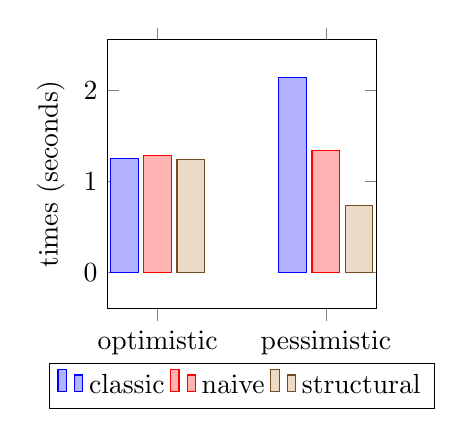
\begin{tikzpicture}
\begin{axis}[
    ybar, ymax = 2, ymin = 0.15,
    enlargelimits=0.3,
    width=5cm, height=5cm,
    legend style={at={(0.5,-0.2)},
      anchor=north,legend columns=-1},
    ylabel={times (seconds)},
    symbolic x coords={optimistic, pessimistic},
    xtick=data
    ]
\addplot coordinates {(optimistic,1.254) (pessimistic,2.142)};
\addplot coordinates {(optimistic,1.282) (pessimistic,1.337)};
\addplot coordinates {(optimistic,1.236) (pessimistic,0.733)};
\legend{classic,naive,structural}
\end{axis}
\end{tikzpicture}
 \captionof{figure}{revers$^o$ forward evaluation \\ for a list with a length of 90}
  \label{fair:plot-reverso}
\end{minipage}%
\begin{minipage}{.5\textwidth}
  \centering
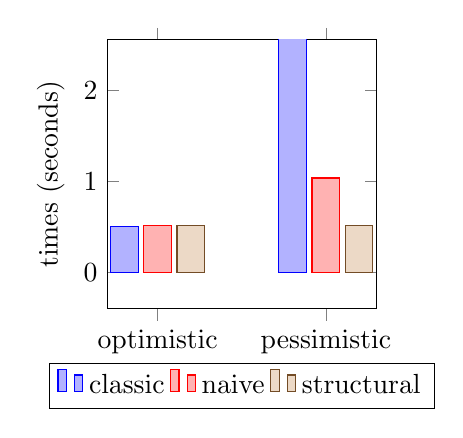
\begin{tikzpicture}
\begin{axis}[
    ybar, ymax = 2, ymin = 0.15,
    enlargelimits=0.3,
    width=5cm, height=5cm,
    legend style={at={(0.5,-0.2)},
      anchor=north,legend columns=-1},
    ylabel={times (seconds)},
    symbolic x coords={optimistic, pessimistic},
    xtick=data
    ]
\addplot coordinates {(optimistic,0.504) (pessimistic,300)};
\addplot coordinates {(optimistic,0.508) (pessimistic,1.035)};
\addplot coordinates {(optimistic,0.513) (pessimistic,0.513)};
\legend{classic,naive,structural}
\end{axis}
\end{tikzpicture}
 \captionof{figure}{sort$^o$ forward evaluation \\ for a list with a length of 5}
\label{fair:plot-sorto}
\end{minipage}
\end{figure*}

\begin{figure*}
\centering
\begin{minipage}{.5\textwidth}
  \centering
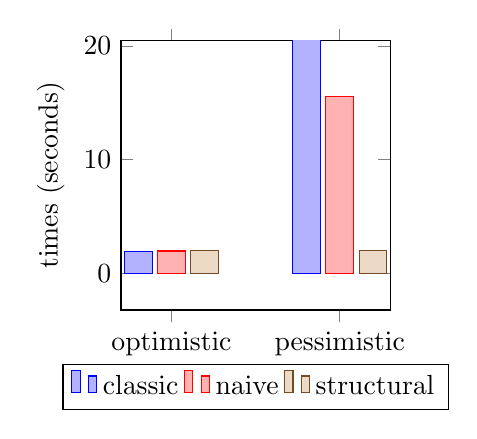
\begin{tikzpicture}
\begin{axis}[
    ybar, ymax = 16, ymin = 1.2,
    enlargelimits=0.3,
    width=5cm, height=5cm,
    legend style={at={(0.5,-0.2)},
      anchor=north,legend columns=-1},
    ylabel={times (seconds)},
    symbolic x coords={optimistic, pessimistic},
    xtick=data
    ]
\addplot coordinates {(optimistic,1.909) (pessimistic,300)};
\addplot coordinates {(optimistic,1.945) (pessimistic,15.516)};
\addplot coordinates {(optimistic,1.980) (pessimistic,1.978)};
\legend{classic,naive,structural}
\end{axis}
\end{tikzpicture}
 \captionof{figure}{``The Tower of Hanoi'' \\ solver evaluation}
\label{fair:plot-hanoi}
\end{minipage}%
\begin{minipage}{.5\textwidth}
  \centering
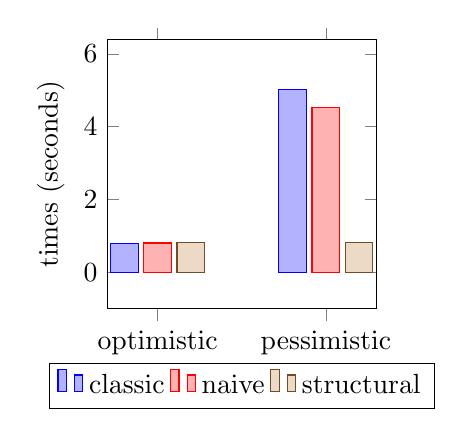
\begin{tikzpicture}
\begin{axis}[
    ybar, ymax = 5, ymin = 0.375,
    enlargelimits=0.3,
    width=5cm, height=5cm,
    legend style={at={(0.5,-0.2)},
      anchor=north,legend columns=-1},
    ylabel={times (seconds)},
    symbolic x coords={optimistic, pessimistic},
    xtick=data
    ]
\addplot coordinates {(optimistic,0.783) (pessimistic,5.019)};
\addplot coordinates {(optimistic,0.801) (pessimistic,4.522)};
\addplot coordinates {(optimistic,0.812) (pessimistic,0.817)};
\legend{classic,naive,structural}
\end{axis}
\end{tikzpicture}
 \captionof{figure}{``Bridge and torch problem'' \\ solver evaluation}
\label{fair:plot-bridge}
\end{minipage}
\end{figure*}

Now we will discuss evaluation. Целью эвалюации является выявления влияния порядка конъюнктов на эффективность трех различных семантик.

Первая семантика с предикатом $pred_{\mbox{\lstinline{true}}}$ близка к классическим реализациям \mk. В дальнейшем будем называть её {\bf left-biased}.

Вторая семантика с предикатом $pred_N$ соответсвует равномерному вычислению всех конъюнктов. Эту семантику будем назвать {\bf naive}.

Третья семантика с предикатом $pred_{\leq_{sr}}$ вычисляет структурно-рекурсивные конъюнкты, пока убывают структурно-рекурсивные аргументы. Её будем называть {\bf structural}.

For evaluation we've chosen two simple programs (list reversing and list sorting) and three more complicated (the ``Hanoi Towers''\footnote{\url{https://en.wikipedia.org/wiki/Tower_of_Hanoi}} solver, the
``Bridge and torch problem''\footnote{\url{https://en.wikipedia.org/wiki/Bridge_and_torch_problem}} solver and ``Water pouring puzzle''\footnote{\url{https://en.wikipedia.org/wiki/Water_pouring_puzzle}} solver).
% Для каждой программы мы сделали две версии. Оптимистичная версия --- это программа, в которой мы вручную подобрали оптимальный порядок конъюнктов и пессиместичная версия --- программа с неоптимальным порядком конъюнктов. В последующих диаграммах и таблице указаны средние значения 10 запусков тестов. Также для наивной равномерной конъюнкции мы подобрали количество разверток вручную. Для равномерной конъюнкции, основанной на структурной рекурсии, N было фиксировано и равно 100.
Each program was written in two versions: ``optimistic'' (with the order of important conjuncts set to provide the best performance) and ``pessimistic'' (with the order of important
conjuncts set to provide the worst performance). Also we evaluated list reversing and list sorting in both directions. In the case of the list reversing, queries \lstinline{(revers$^o$ [1;2;3] q)} and \lstinline{(revers$^o$ q [1;2;3])}\! will give the same answer \lstinline{q = [3;2;1]} but the ``optimistic'' order of conjuncts is different for them. In the case of list sorting, queries \lstinline{(sort$^o$ [1;2;3] q)} and \lstinline{(sort$^o$ q [1;2;3])} will give different answers. The first one gives sorted list \lstinline{q = [1;2;3]}, the second one gives all permutations of list \lstinline{[1;2;3]}\!\!. 

All benchmarks were run ten times, and the average time was taken. For the naive  semantics we cherry-picked the best value of unfolding bound manually. Structural arguments for each relations were detected automatically.

% На изображениях 12-15 представлены результаты апробации в виде столбцовых диаграмм. В оптимистичном случае результаты схожи для всех семантик. В пессиместичном случае время работы напрпавленной конъюнкции резко возрастает, время работы наивной равномерной конъюнкции также ворзрастает, но не так сильно. Равномерная конъюнкция, основанная на структурной рекурсии, демострирует схожую эффективность в сравнении с оптимистичным случаем.
Fig.~\ref{fair:plot-reverso}-\ref{fair:plot-bridge} show the results of evaluation in the form of bar charts. In the optimistic case, the results are similar for all semantics.
In the pessimistic case the evaluation time of the directed conjunction rapidly increases, the evaluation time of the naive fair conjunction also increases, but not so much.
The fair semantics based on structural recursion demonstrates a similar efficiency as in the optimistic case.

\begin{figure*} %[h!]
  \small
  \centering
  \begin{tabular}{ c | c | c | c | c | c | c | c }
    \multirow{2}{*}{relation} & \multirow{2}{*}{size} & 
    \multicolumn{2}{c}{left-biased semantics} &
    \multicolumn{2}{c}{naive semantics} &
    \multicolumn{2}{c}{structural semantics} \\
    \cline{3-8}
    & & optimistic & pessimistic & optimistic & pessimistic & optimistic & pessimistic  \\ 
    \hline
    \multirow{3}{*}{\begin{tabular}{c} forward \\ revers$^o$ \end{tabular}}
                 & 30   & 0.527 & 0.587  & 0.532 & 0.595   & 0.539 & 0.532 \\
                 & 60   & 0.639 & 0.947  & 0.643 & 0.790   & 0.657 & 0.577 \\
                 & 90   & 1.254 & 2.142  & 1.282 & 1.337   & 1.236 & 0.733 \\
    \hline
    \multirow{3}{*}{\begin{tabular}{c} backward \\ revers$^o$ \end{tabular}}
                 & 30   & 0.531 & 0.579  & 0.547 & 0.570  & 0.553 & 0.563 \\
                 & 60   & 0.655 & 0.875  & 0.667 & 0.812  & 0.668 & 0.681 \\
                 & 90   & 1.316 & 1.813  & 1.327 & 1.503  & 1.360 & 1.359 \\
    \hline
    \multirow{5}{*}{\begin{tabular}{c} forward \\ sort$^o$ \end{tabular}}
                 & 3    & 0.467 & 0.503  & 0.474 & 0.481  & 0.472 & 0.479 \\
                 & 4    & 0.484 & 4.679  & 0.485 & 0.493  & 0.490 & 0.488 \\
                 & 5    & 0.504 & $>$300 & 0.508 & 1.035  & 0.513 & 0.513 \\
                 & 6    & 0.526 & $>$300 & 0.237 & 14.369 & 0.544 & 0.547 \\
                 & 30   & 1.915 & $>$300 & 1.936 & $>$300 & 1.983 & 1.987 \\
    \hline
    \multirow{4}{*}{\begin{tabular}{c} backward \\ sort$^o$ \end{tabular}}
                 & 3    & 0.518 &  0.519 & 0.518 & 0.521  & 0.520 & 0.521 \\
                 & 4    & 0.533 &  0.856 & 0.534 & 0.540  & 0.534 & 0.537 \\
                 & 5    & 0.680 & 93.914 & 0.713 & 1.528  & 0.718 & 0.714 \\
                 & 6    & 2.931 & $>$300 & 2.947 & 59.647 & 2.938 & 2.936 \\
    \hline
    hanoi$^o$    & -    & 1.909 & $>$300 & 1.945 & 15.516 & 1.980 & 1.978 \\
    \hline
    bridge$^o$   & -    & 0.783 & 5.019  & 0.801 & 4.522  & 0.812 & 0.817 \\
    \hline
    water$^o$    & -    & 3.513 & $>$300 & 3.518 & $>$300 & 3.538 & 3.771

  \end{tabular}
  \caption{The results of evaluation: running times of benchmarks in seconds}
  \label{fair:evaluation-table}
\end{figure*}

% Более подробно результаты представлены на изображении 16. Можно заметить, что время работы программы sorto в пессиместичном случае очень быстро растет с увеличением длины списка для направленной конъюнкции и наивной равномерной. В случае с равномерной конъюнкцией, основанной на структурной рекурсии, пессиместичный случай растет сопостовимо с оптимистичным.
The results are presented in more detail in Fig.~\ref{fair:evaluation-table}. ``Hanoi Towers'' solver has name \lstinline{hanoi$^o$}, ``Bridge and torch problem'' solver has name \lstinline{bridge$^o$} and ``Water pouring puzzle'' solver has name \lstinline{water$^o$}. We can conclude that forward and backward \lstinline{sort$^o$} runtime in the pessimistic case increases very rapidly with increasing the list length for left-biased and naive fair semantics. In the case of the fair semantics based on structural recursion the running time in pessimistic case increases on a par with that in the optimistic one. Also the solver \lstinline{water$^o$} very slow in the pessimistic case for left-biased and naive fair. However, fair conjunction based on structural recursion pessimistic case is no different from an optimistic case.


% Подводя итог, равномерная конъюнкция, основанная на структурной рекурсии сопоставима по эффективности с направленной конъюнкцией. Более того, это конъюнкция слабо зависит от порядка конъюнктов.
To summarize, the fair semantics based on structural recursion does not introduce any essential overhead in comparison with left-biased semantics in an optimistic case. At the same time it
weakly depends on the order of the conjuncts, and thus demonstrates much better performance in the pessimistic case.

\section{Conclusion}
\label{conclusion}

We presented an approach for converting typed functional programs into relations. Relational conversion 
in many cases allows us to avoid tedious recoding of functional specifications into relational form and to 
concentrate on writing relational specifications only when their reconstruction from functions is impossible or 
undesirable. Our implementation works for the subset of OCaml; we evaluated it for a number of interesting 
examples and acquired some new relational solutions.

There is a number of directions for future research. First, a performance evaluation is desirable~--- at
present time we do not know, what slowdown factor is. Another problem is a development of an approach to
prove complete correctness (or refute this claim).


\bibliographystyle{ACM-Reference-Format}
\bibliography{fair-conj}


\end{document}
\endinput

